\documentclass[xetex]{beamer}

\usepackage[english]{babel}
\usepackage{polyglossia}
\setdefaultlanguage{french}
\usepackage{graphicx}
\usepackage{adjustbox}
\usepackage{tikz, pgfplots}
\usetheme{modern}



\title
    {Architecture des systèmes d'information}
\subtitle
    {Gestion des contacts d'une banque}
\author
    {H4401}


\begin{document}

    \frame[plain]{\titlepage}

    \frame{\tableofcontents}

    \section{Découpage MCD et objets métier}
     \begin{frame}{Découpage MCD (1)}
	
\noindent\makebox[\textwidth]{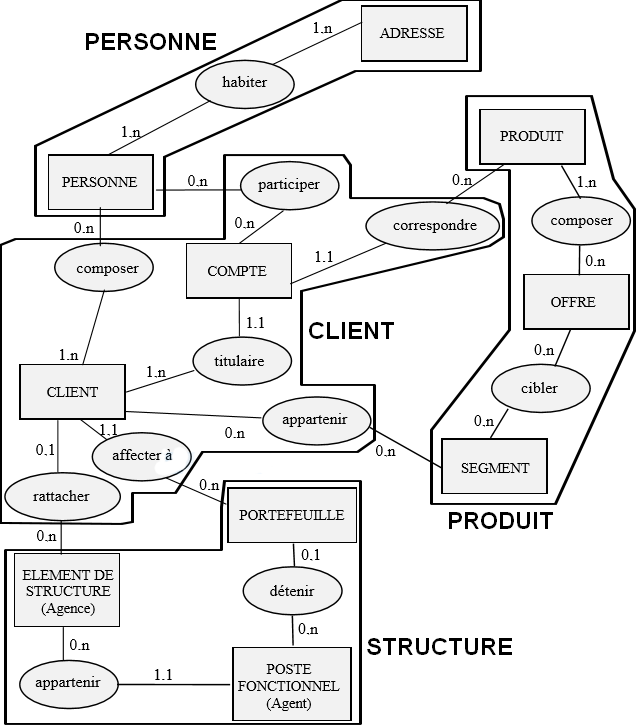
\includegraphics[height=8cm]{../report/figures/mcd/MCD_Clients_Produits.png}}

    \end{frame}
    \begin{frame}{Découpage MCD (2)}
\noindent\makebox[\textwidth]{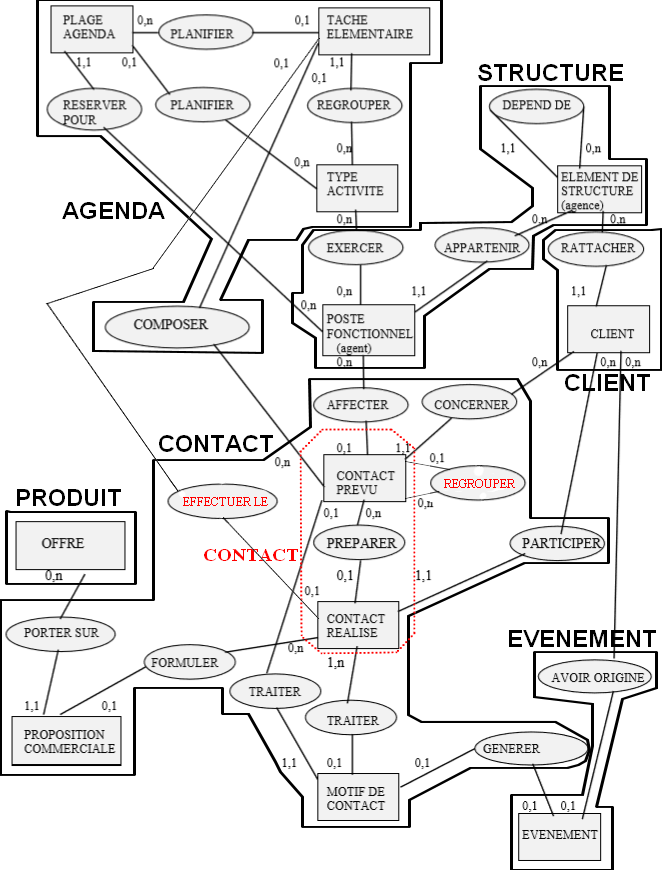
\includegraphics[height=8cm]{../report/figures/mcd/MCD_Commercial.png}}
    \end{frame}
    \section{Diagramme d’état}
    \begin{frame}{Diagramme d'état de l'objet contact}
\noindent\makebox[\textwidth]{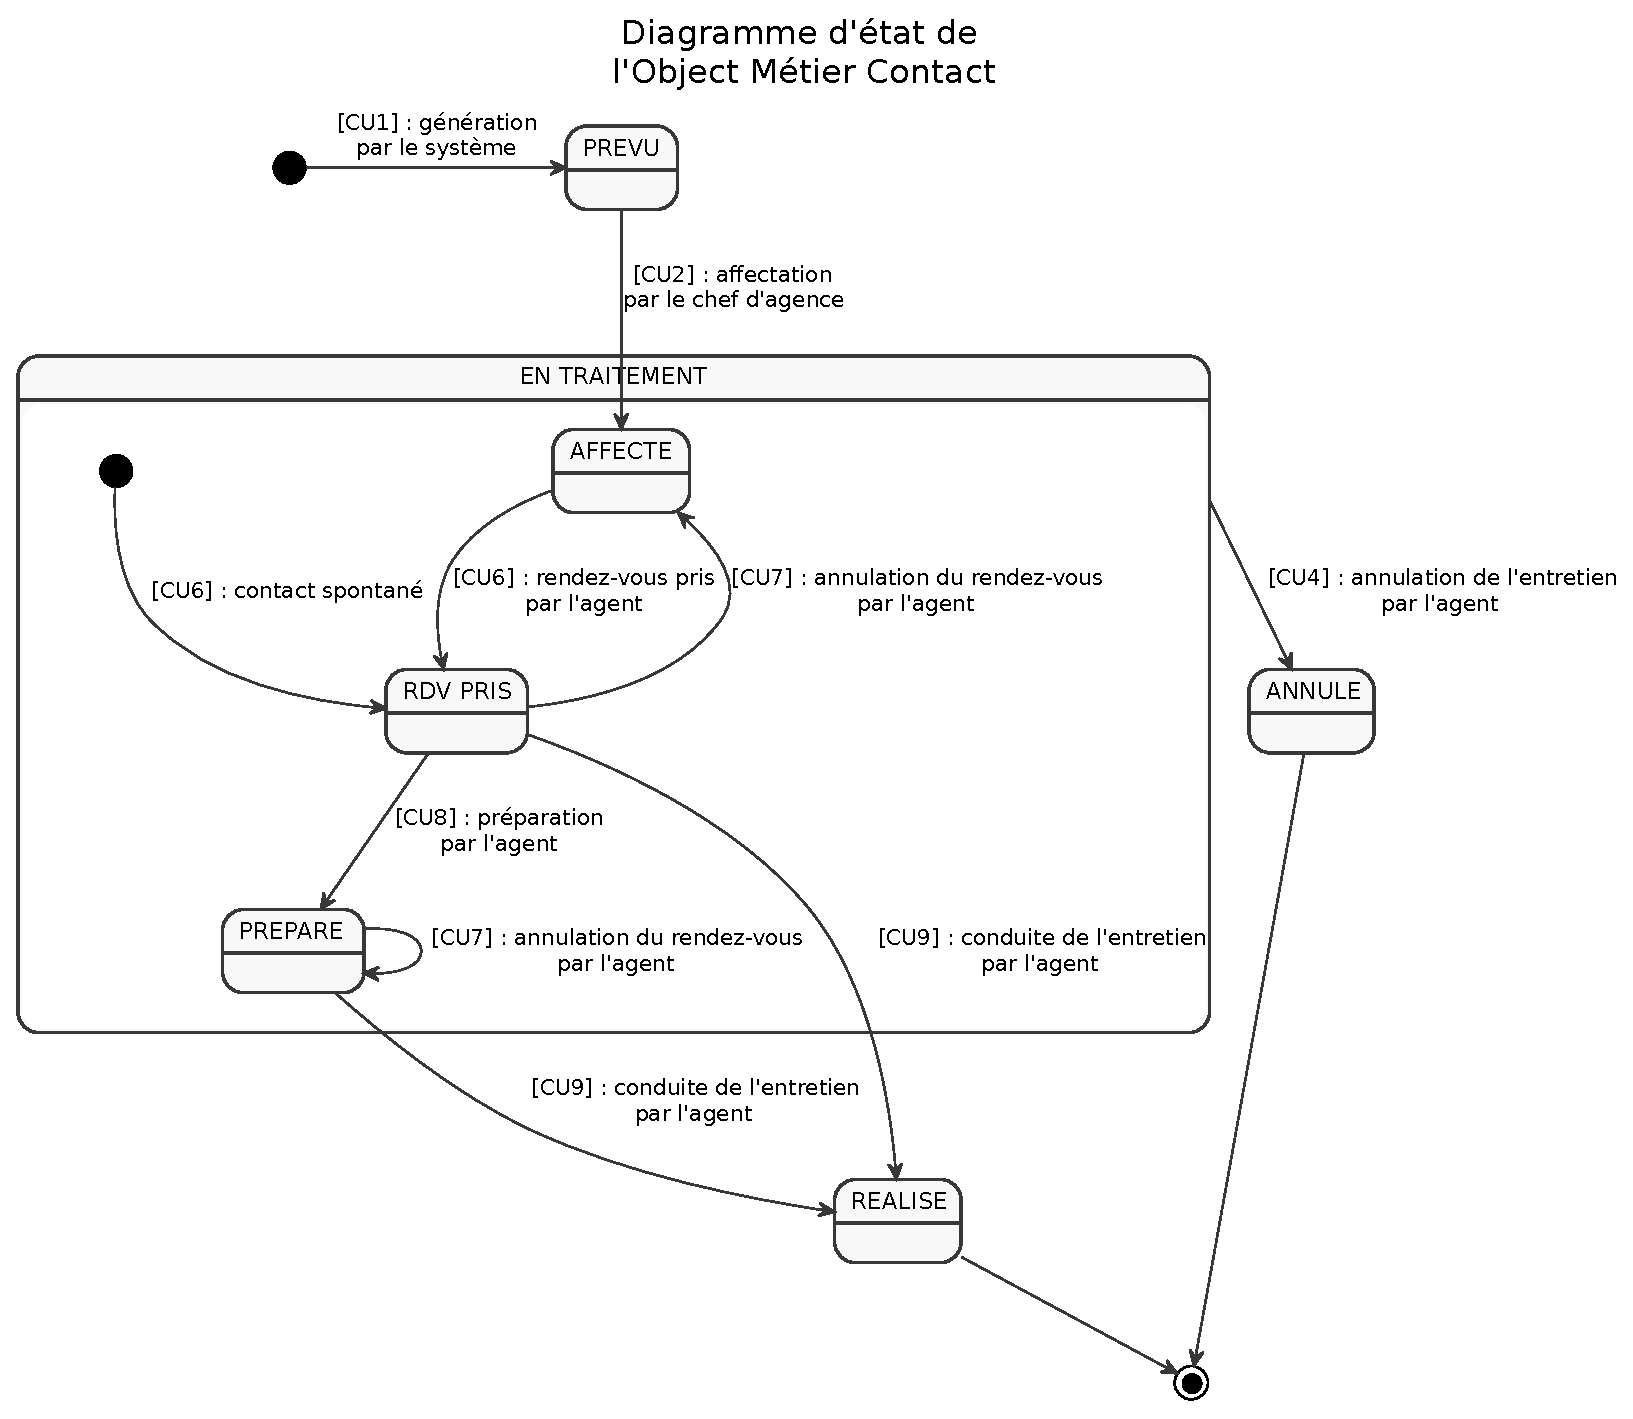
\includegraphics[height=8cm]{../report/figures/eps/diag_etats_contact}}
    \end{frame}
    \section{IHM Agenda}

 \begingroup
        \setbeamercolor{background canvas}{parent=palette secondary}
        \begin{frame}[plain]
            \centering
            \vfill
            \usebeamerfont{section title}\usebeamercolor[fg]{frametitle}IHM Agenda
            \vfill
        \end{frame}
    \endgroup    
    
    \section{Diagramme de séquence détaillé - CU7}
    \begin{frame}{Diagramme de séquence détaillé - CU7}
    \adjustbox{width=1.1\textwidth, center, trim={0} {.43\height} {0} {0},clip}%
  {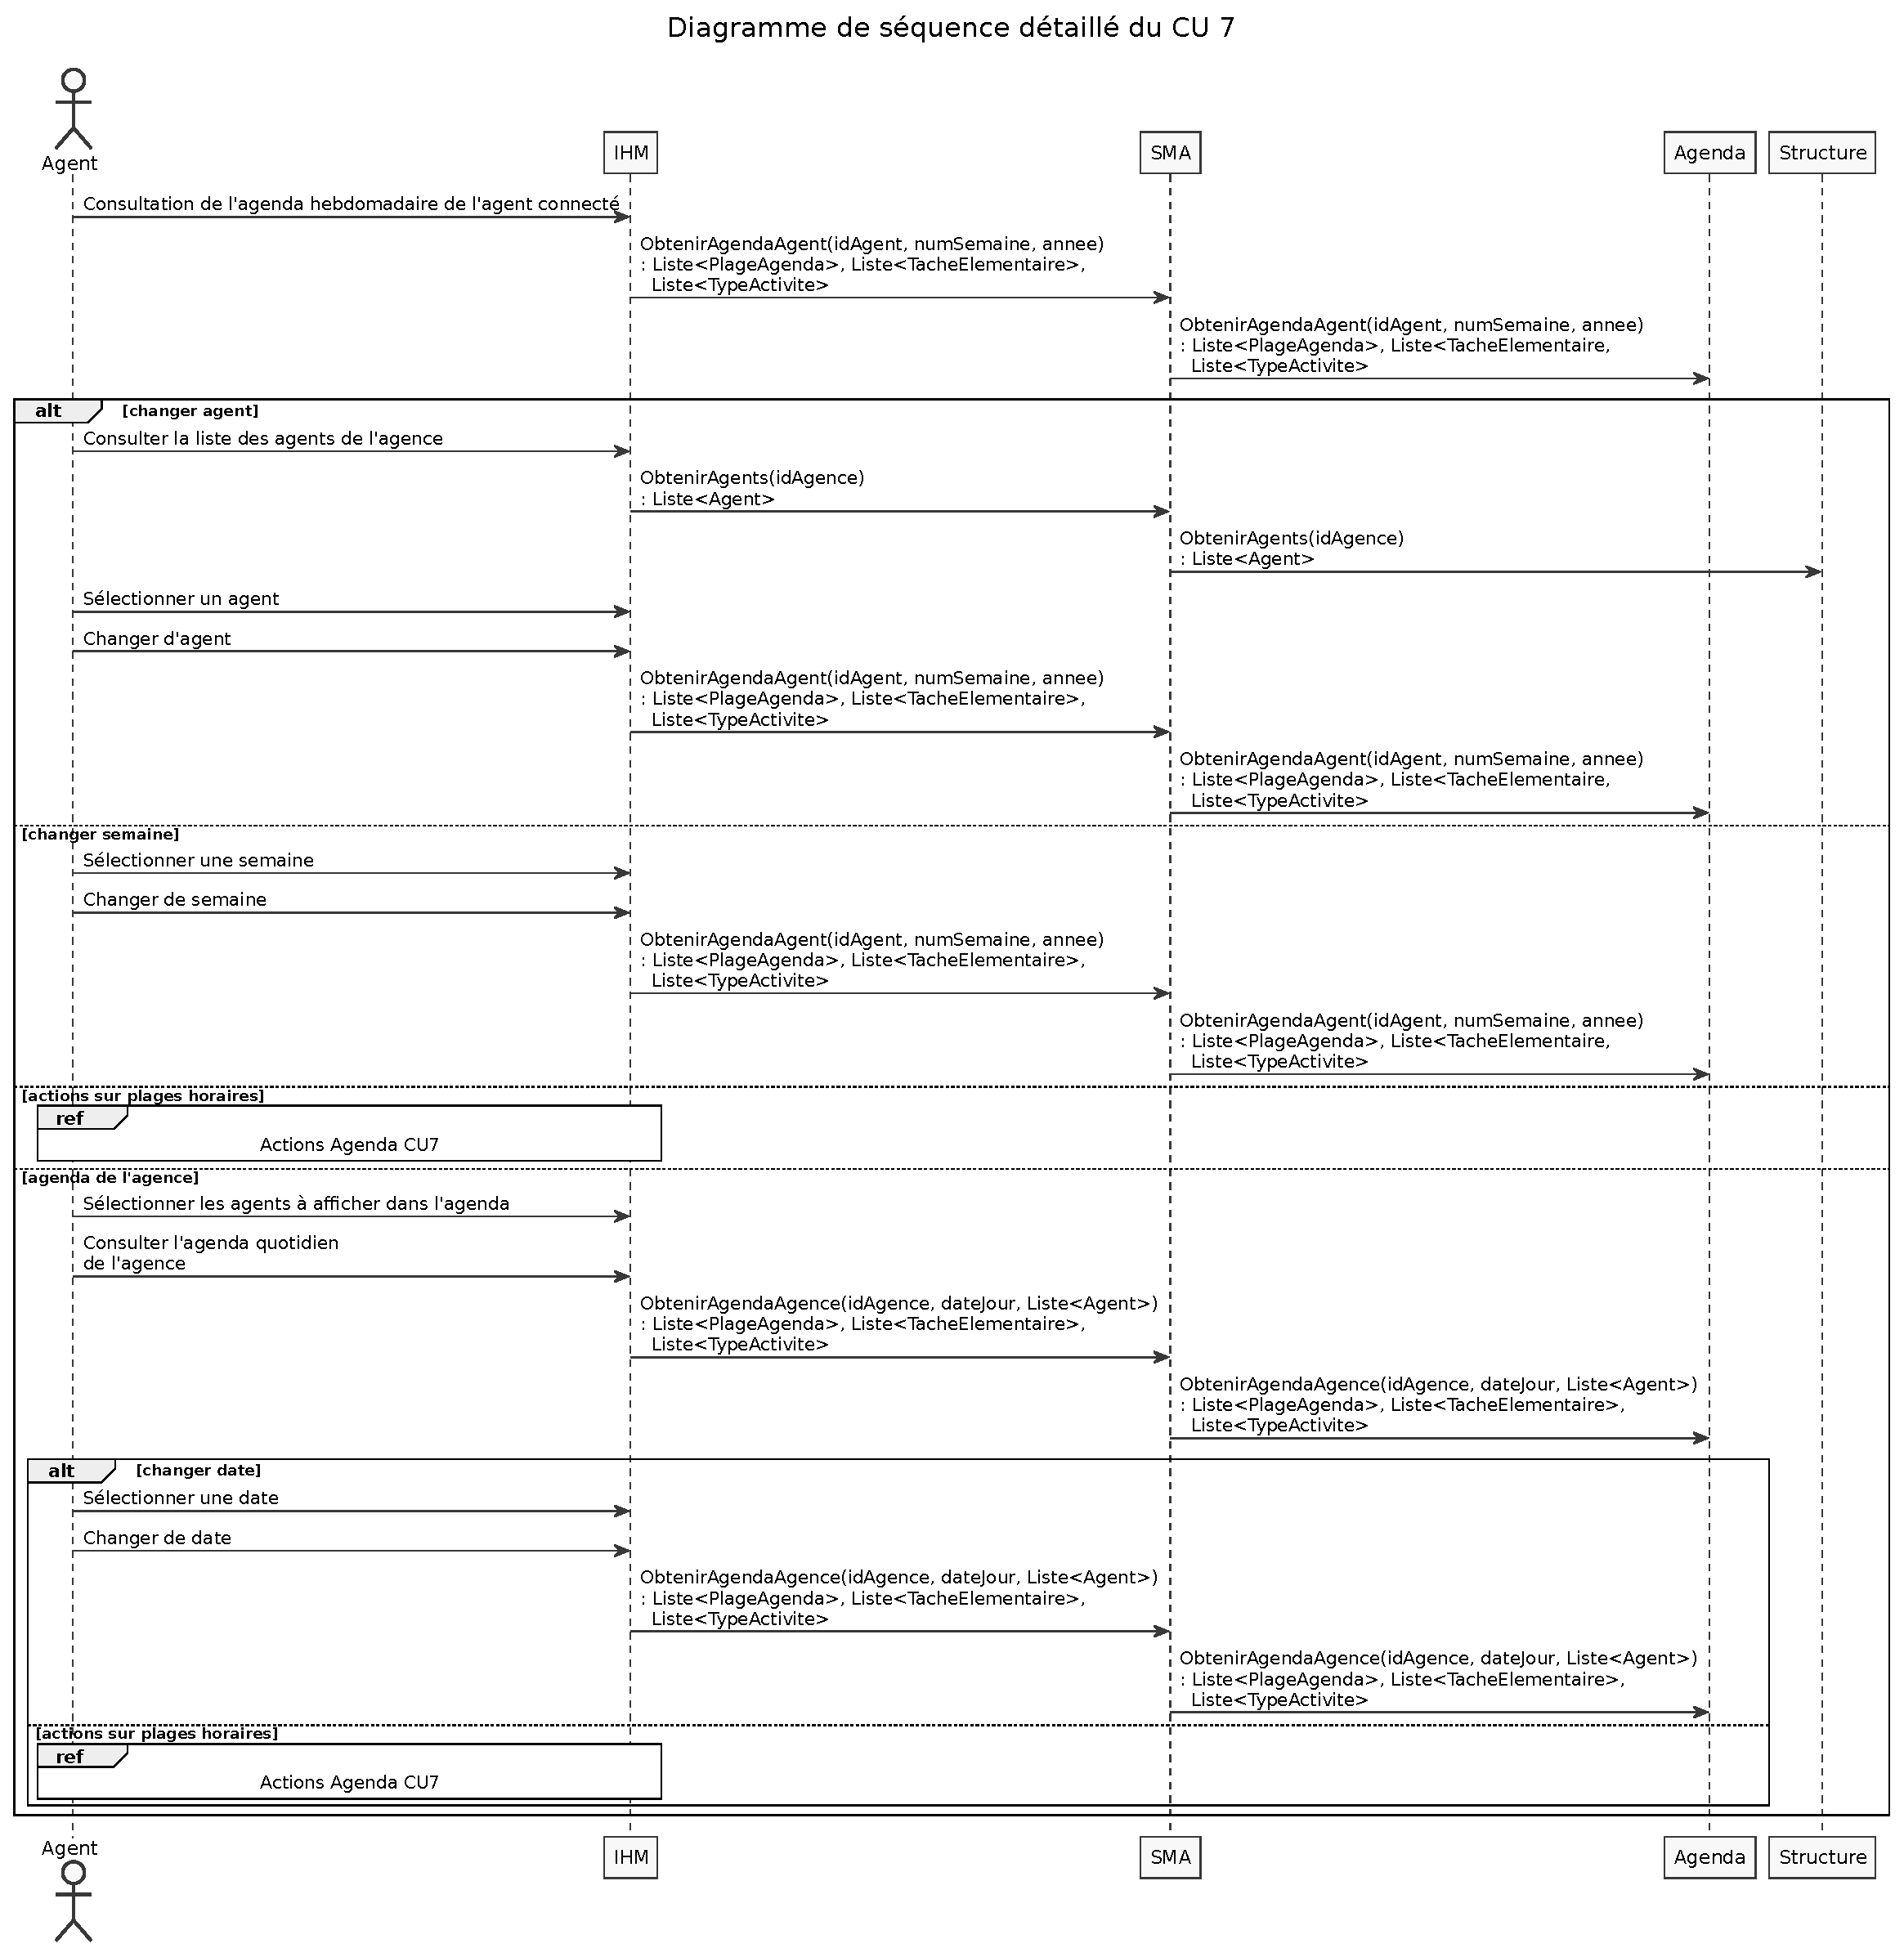
\includegraphics[height=12cm]{../report/figures/eps/DSD_CU7}}
    \end{frame}
    
    
        \begin{frame}{Diagramme de séquence détaillé- CU7}
    \adjustbox{width=1.1\textwidth, center, trim={0} {0} {0} {.5\height},clip}%
  {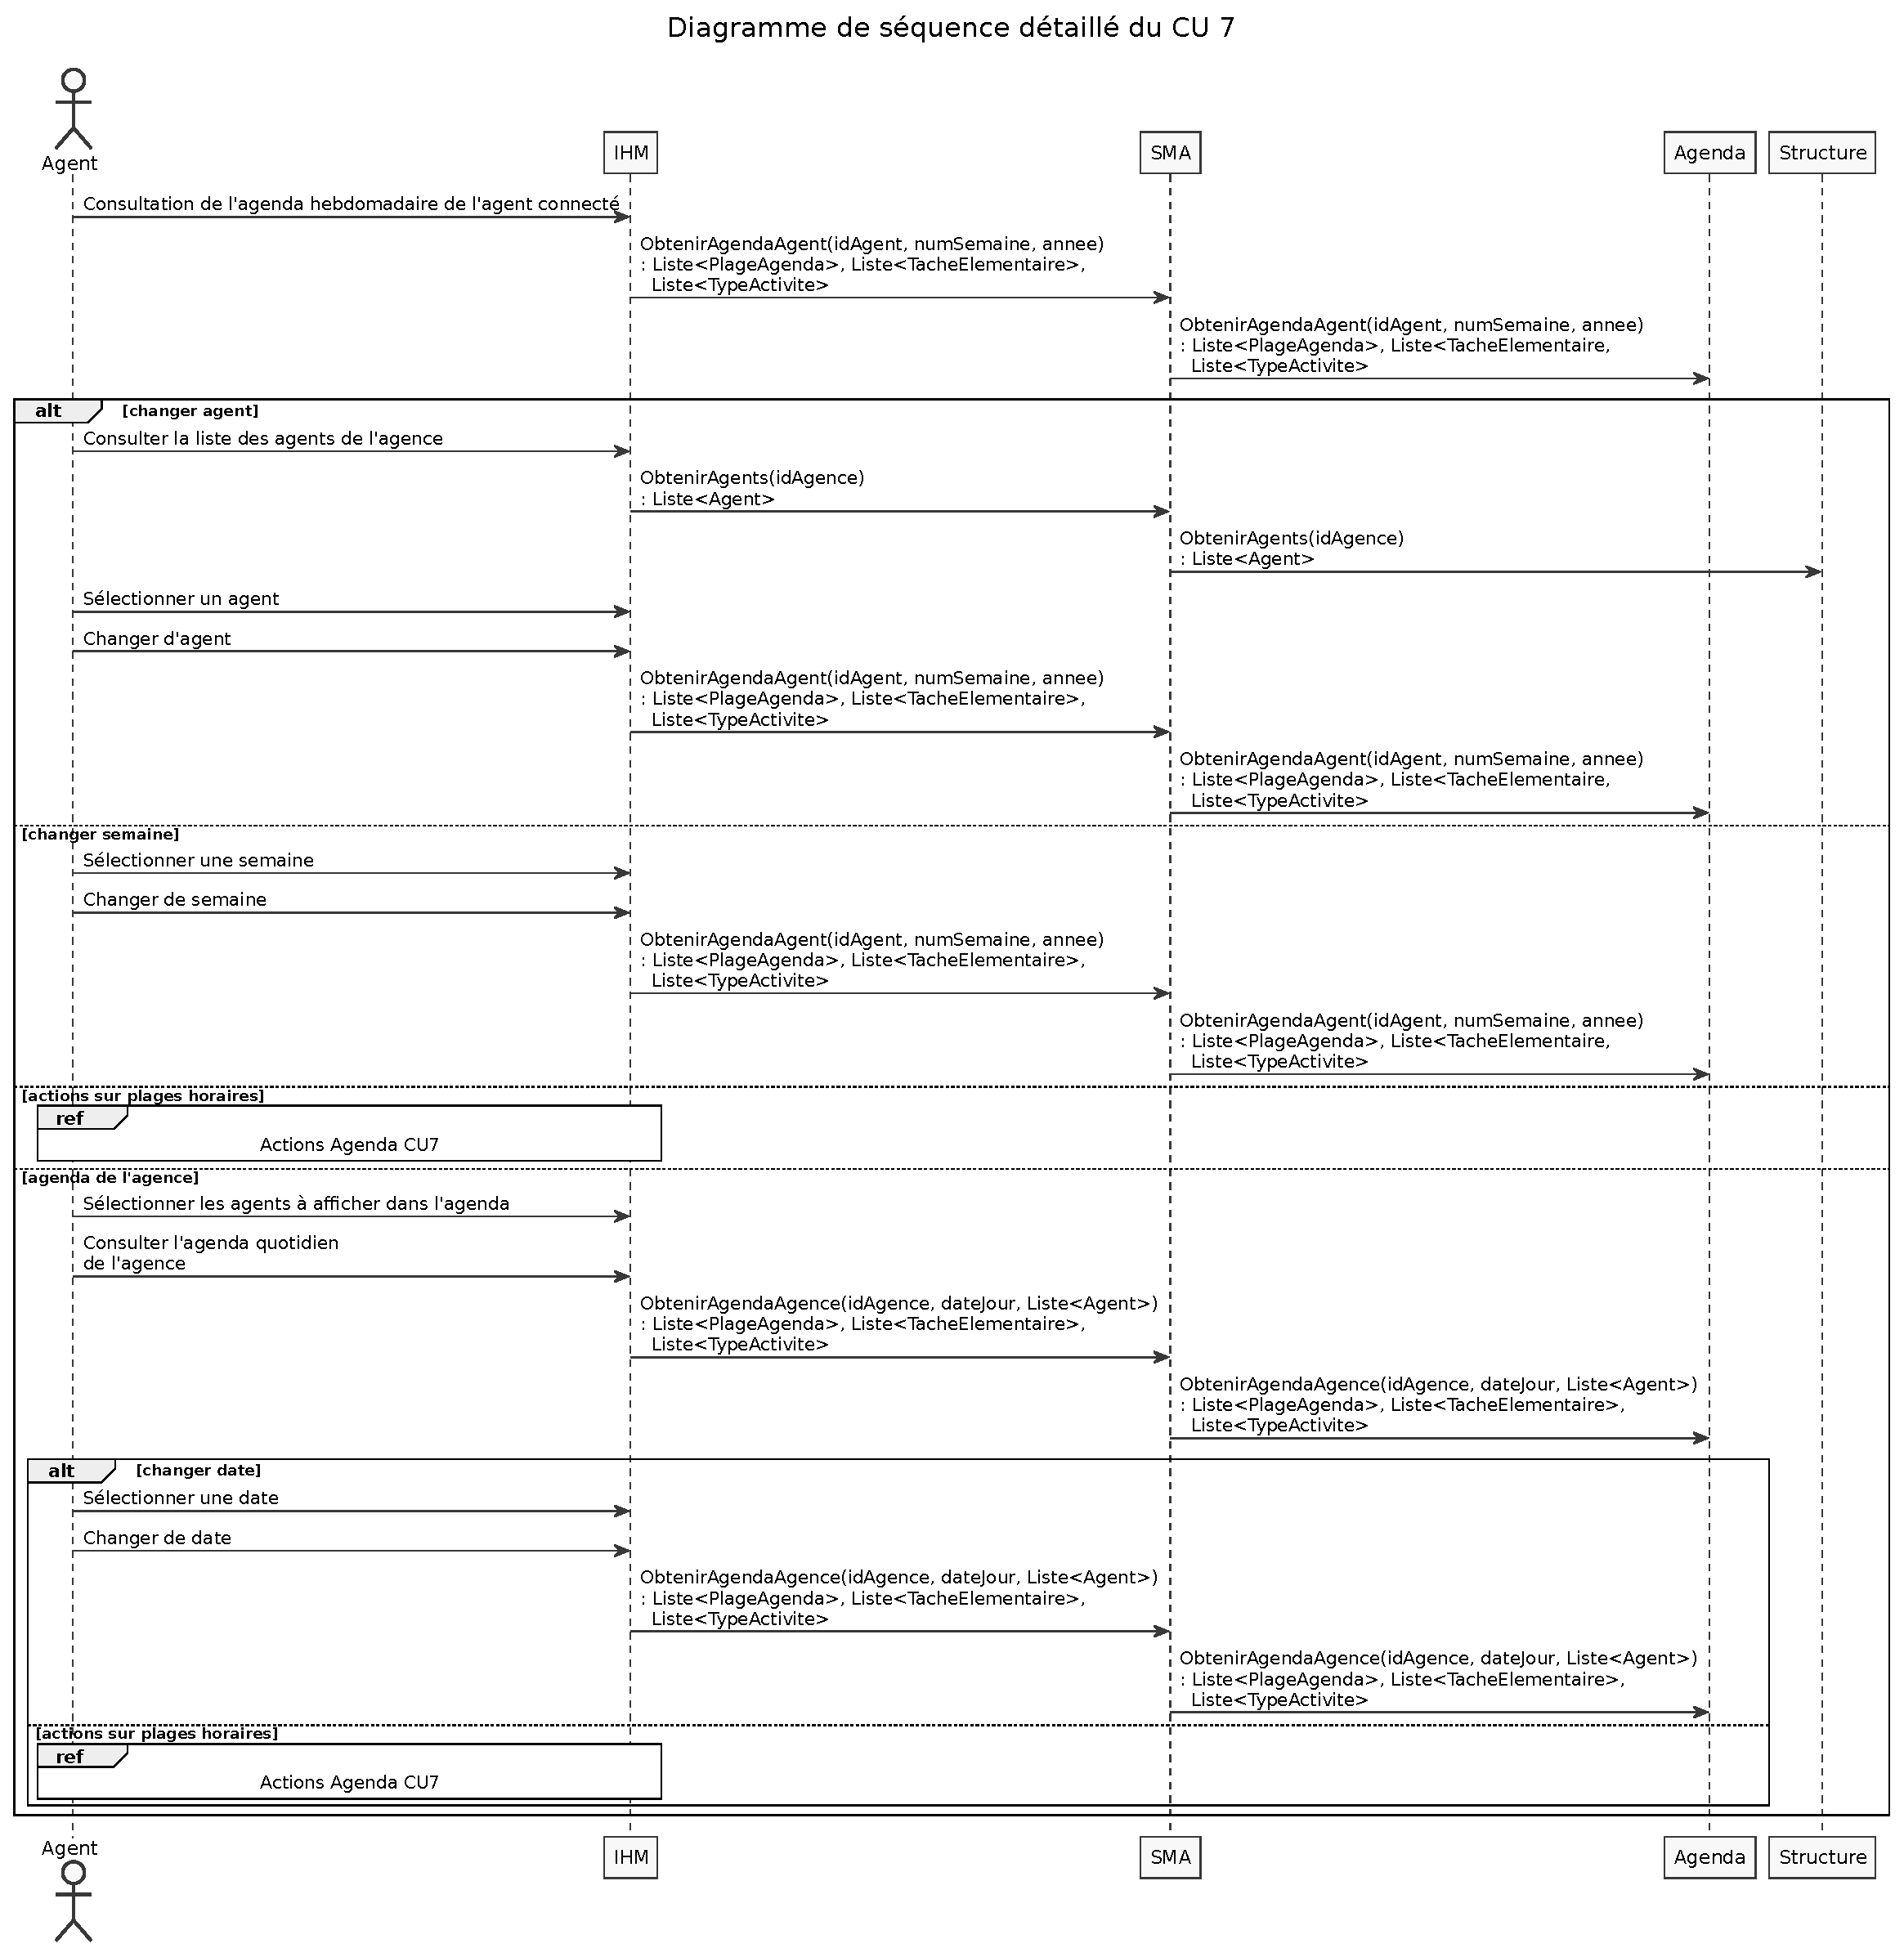
\includegraphics[height=12cm]{../report/figures/eps/DSD_CU7}}
    \end{frame}
    
    \begin{frame}{Diagramme de séquence détaillé - Action Agenda}
    \adjustbox{width=1.1\textwidth, center, trim={0} {.5\height} {0} {0},clip}%
  {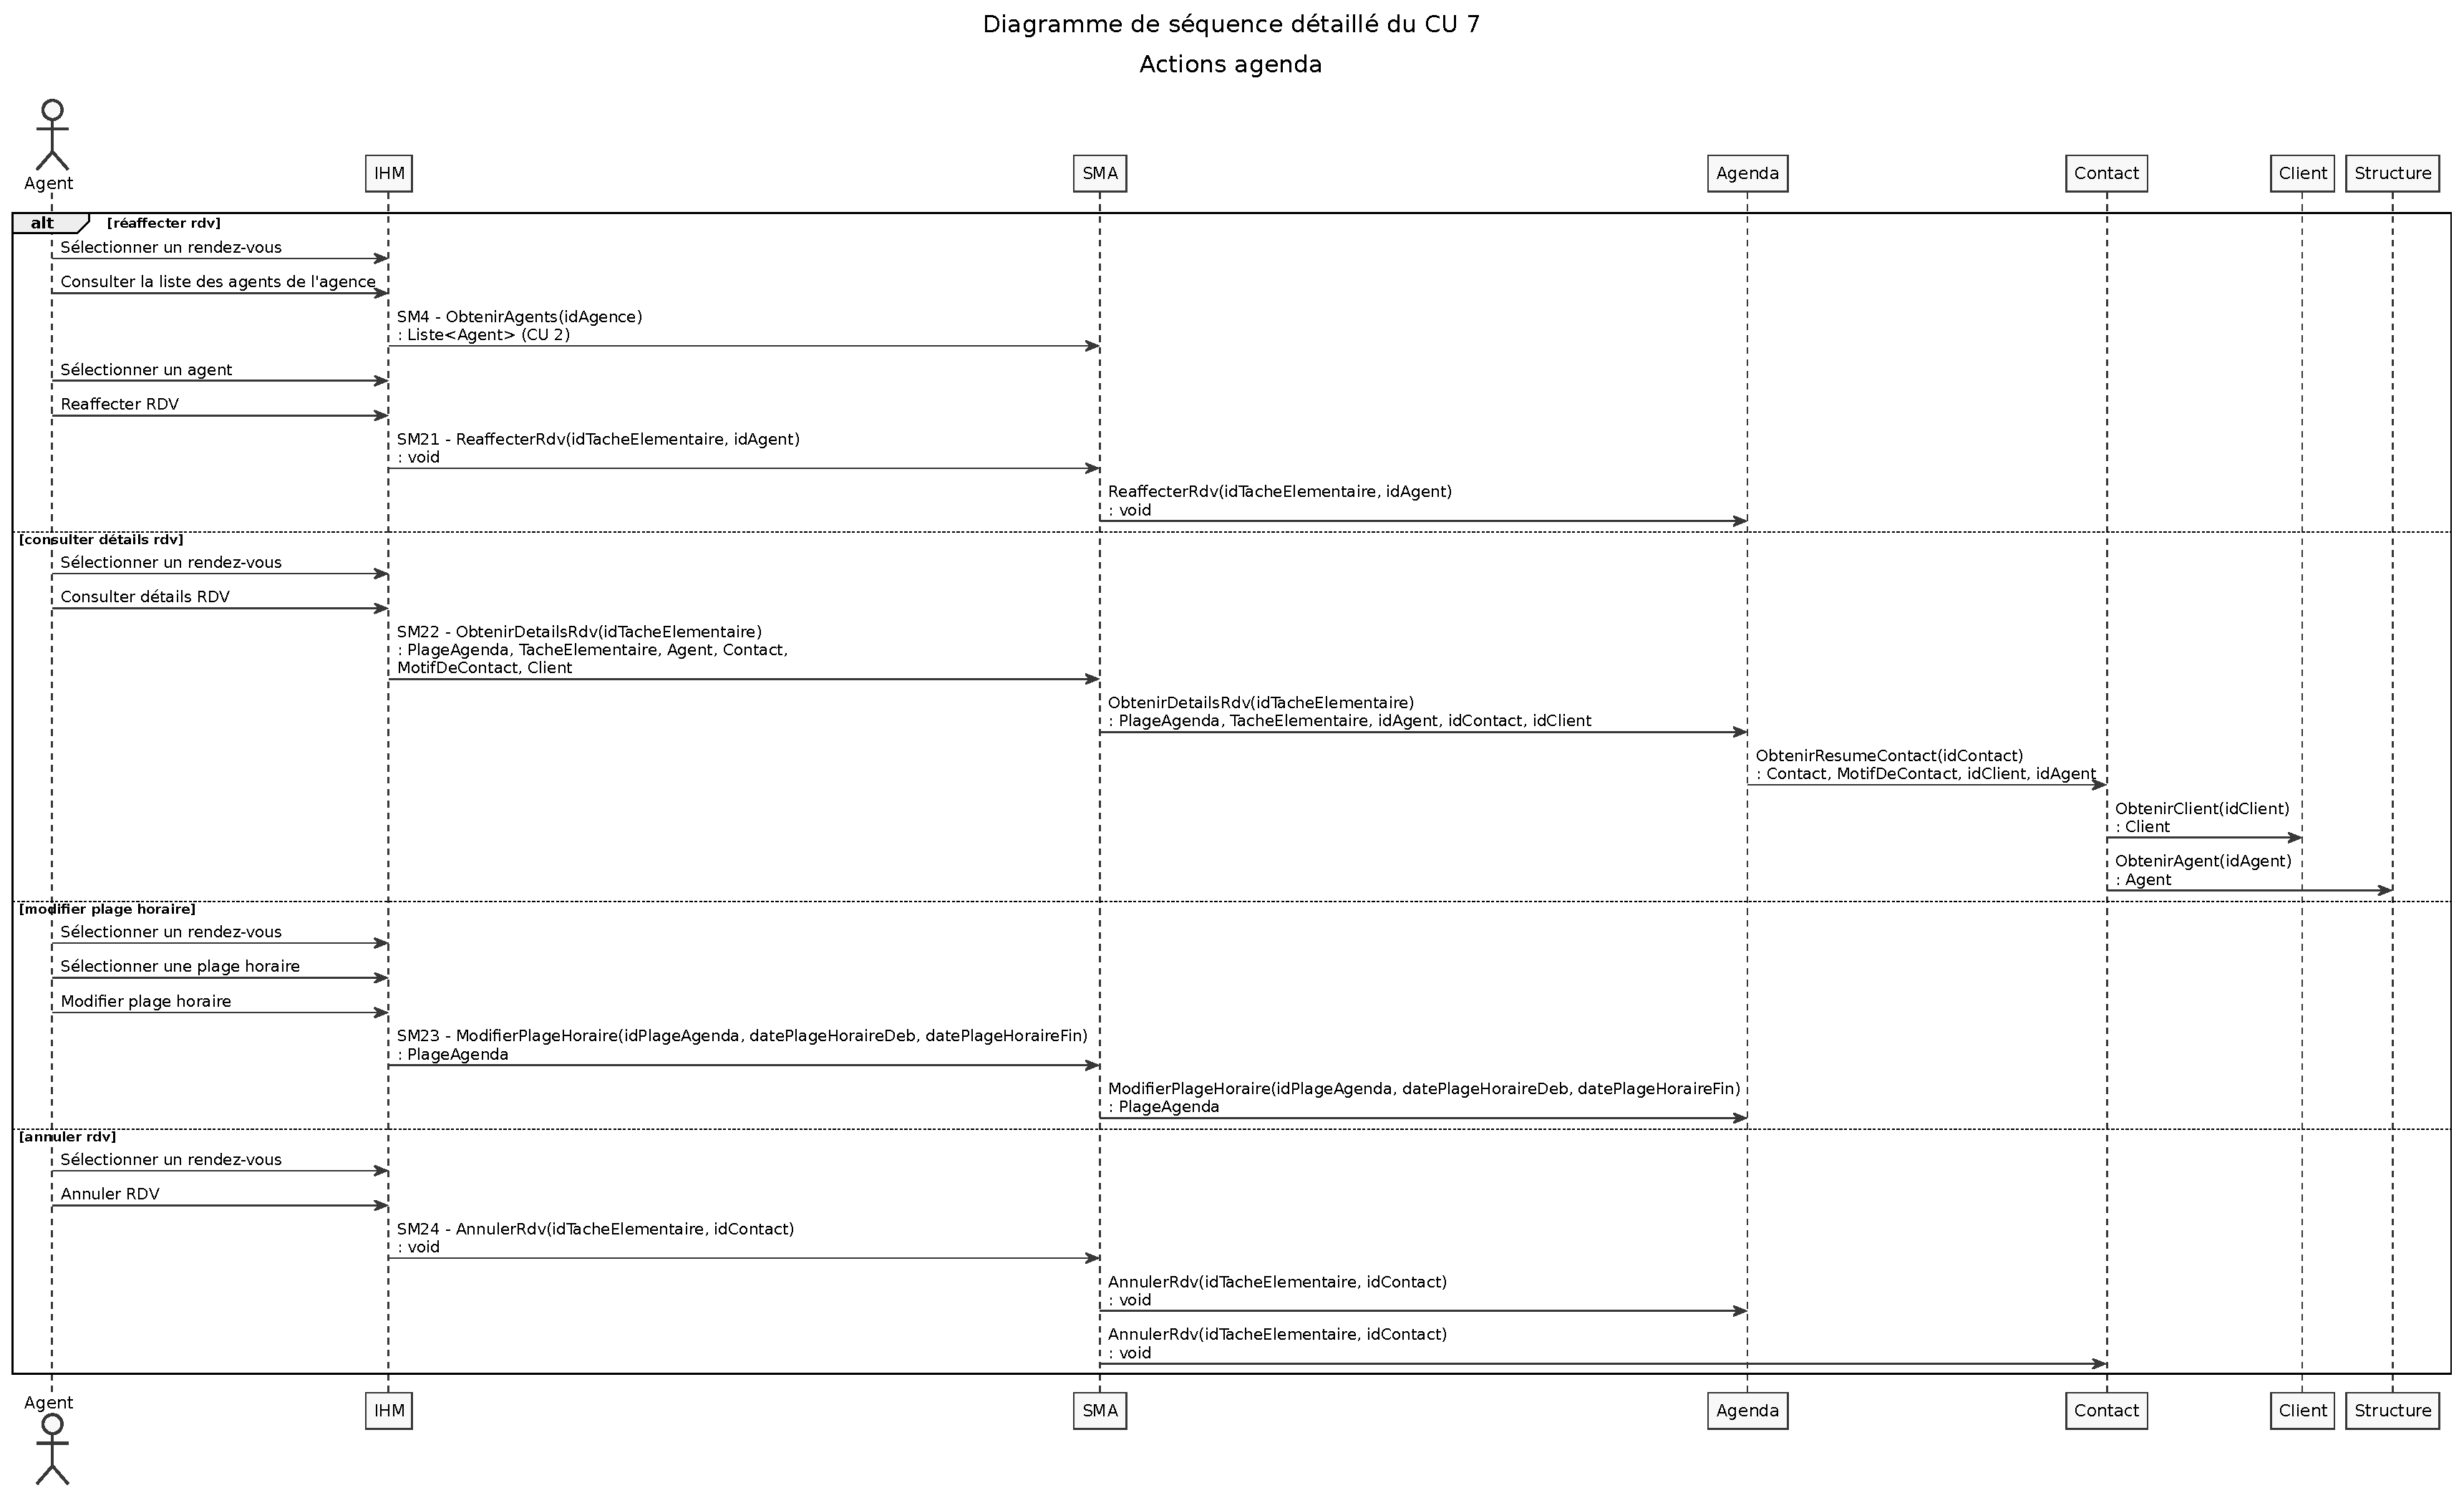
\includegraphics[height=12cm]{../report/figures/eps/DSD_CU7_ActionsAgenda}}
    \end{frame}
    
     \begin{frame}{Diagramme de séquence détaillé - Action Agenda}
    \adjustbox{width=1.1\textwidth, center, trim={0} {0} {0} {.5\height},clip}%
  {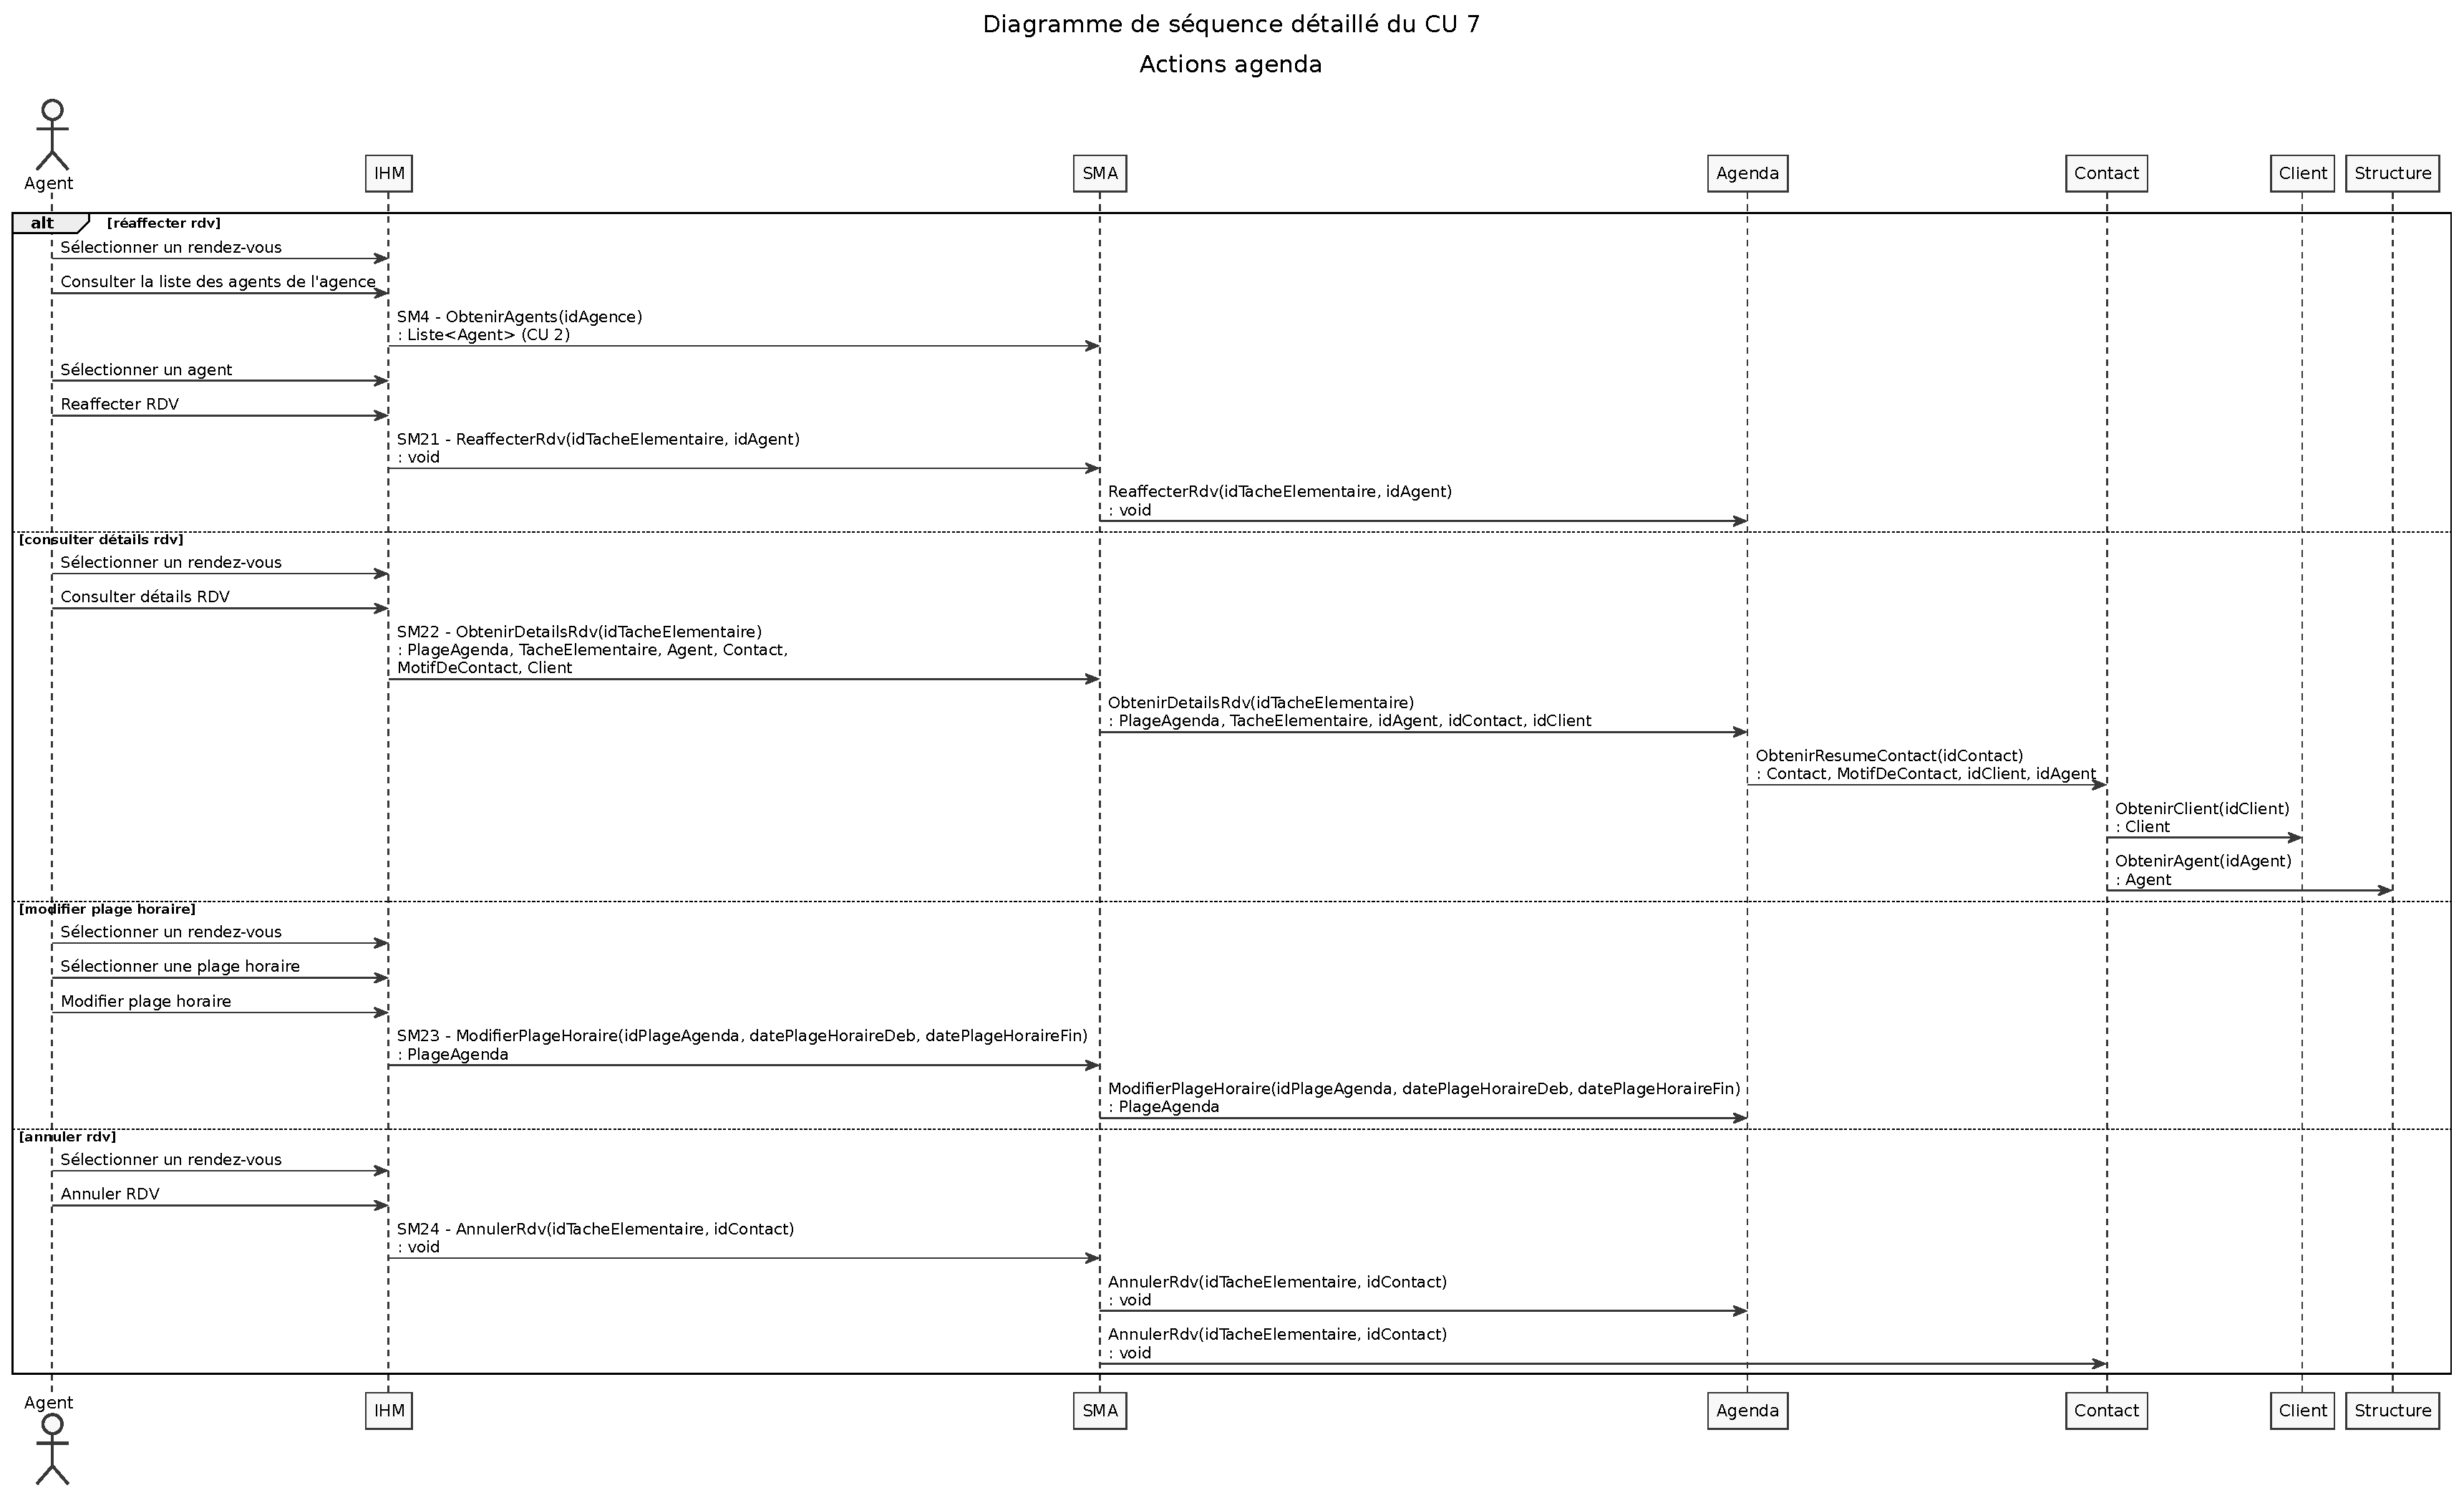
\includegraphics[height=12cm]{../report/figures/eps/DSD_CU7_ActionsAgenda}}
    \end{frame}
    
    
    \section{Diagramme de collaboration}
    \begin{frame}{Diagramme de collaboration}
\begin{block}{Todo}
            Inserer le diagramme de collaboration
        \end{block}
    \end{frame}
    
    \section{2 SM + SOM}
    \begin{frame}{SMA - Obtenir Détail Agent}
        \begin{block}{SOM}
            description
        \end{block}
    \end{frame}
    \begin{frame}{SMA - Obtenir détails rdv}
    \begin{block}{SOM}
            description
        \end{block}
    \end{frame}
    
    \begin{frame}{Bilan du projet}
  \begin{figure}
    \begin{tikzpicture}
      \begin{axis}[
        mbarplot,
        ylabel=Temps (Heures),
        axis y line=left,
        axis x line=bottom,
        xmin=0, xmax=5,
        ymin=0, ymax=40,
        xtick={1,2,3,4},
        xticklabels={Conception\\ d’ensemble,Conception\\ fonctionnelle\\ détaillée,Conception\\ applicative\\ détaillée,Architecture\\ technique},%<--Here
        xlabel style={yshift=-1cm},
        x tick label style={
            rotate=62,
            anchor=east,
            font=\footnotesize,
            align=right
        },
        width=\textwidth,
        height=7cm,
      ]

      \addplot plot coordinates {(1, 20) (2, 25) (3, 22.4) (4, 12.4)};
      \addplot plot coordinates {(1, 18) (2, 24) (3, 23.5) (4, 13.2)};

      \legend{Temps estimé, Temps passé}

      \end{axis}
    \end{tikzpicture}
  \end{figure}
\end{frame}

\end{document}
